\section{B) Support Vector Machines}

\subsection{i) Train an SVM model}
Support vector machines find the hyperplane that maximises the separation between classes in the feature space. The SVM optimisation objective is to maximise the margin, ie the distance between the decision boundary and the nearest training points (support vectors) from each class. This is achieved by minimising $\frac{1}{2}\|w\|^2$.

Just like the logistic regression model, the sklearn library and it's LinearSVC class was used in this implementation \cite{sklearn_svm}. The LinearSVC class by default uses l2 regularisation, and takes a penalty parameter C.     

The strength of this l2 regularisation is inversely proportional to C, meaning smaller C values result in stronger regularisation, while larger C values result in weaker regularisation.
A wide range of C values were used in order to effectively visualise the impact of the regularisation strength on the model. The following table shows the model parameters for different values of C.

% Confirm these are indeed the models
\begin{table}[H]
    \centering
    \begin{tabular}{c|c|c|c}
        \toprule
        $C$ & Intercept $[w_0]$ & Coefficients $[w_1, w_2]$ & Model \\
        \midrule
        0.0001 & 0.0622 & $[-0.0036,\ 0.0739]$ & $f(x_1, x_2) = 0.0622 - 0.0036x_1 + 0.0739x_2$ \\
        0.001 & 0.2424 & $[-0.0180,\ 0.4671]$ & $f(x_1, x_2) = 0.2424 - 0.0180x_1 + 0.4671x_2$ \\
        1     & 0.6448 & $[-0.0734,\ 1.8435]$ & $f(x_1, x_2) = 0.6448 - 0.0734x_1 + 1.8435x_2$ \\
        100   & 0.6522 & $[-0.0743,\ 1.8623]$ & $f(x_1, x_2) = 0.6522 - 0.0743x_1 + 1.8623x_2$ \\
        \bottomrule
    \end{tabular}
    \caption{SVM model parameters for different values of $C$}
    \label{tab:svm_params}
\end{table}

\subsection{ii) Predict target values}

\begin{figure}[H]
    \centering
    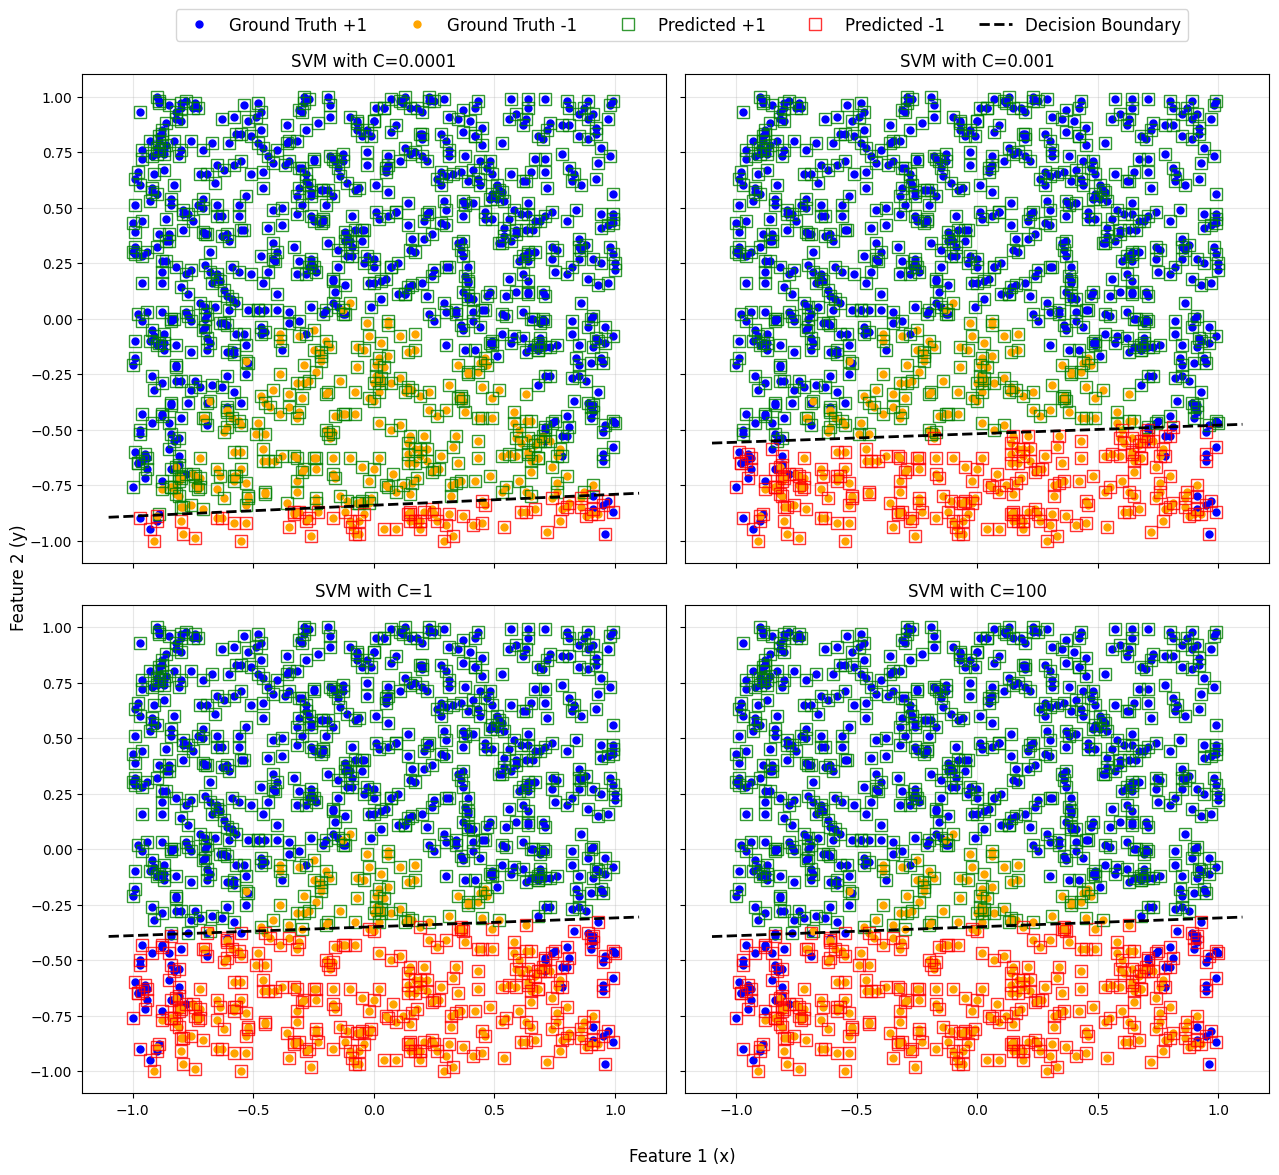
\includegraphics[width=1\textwidth]{figures/SVM_combined1.png}
    \caption{SVM Predictions for different values of C}
    \label{fig:SVM_combined}
\end{figure}

Figure \ref{fig:SVM_combined} shows the SVM predictions for different values of C in a similar fashion to previously. The ground truth is represented by blue and orange point markers, and predictions are overlaid via square markers. The decision boundary is depicted by the black dashed line and was calculated as before.

\subsection{iii) Discuss the impact of C}

\begin{table}[H]
    \centering
    \begin{tabular}{c|c|c|c|c}
        \toprule
        $C$ & Accuracy & Precision & Recall & F1-Score \\
        \midrule
        0.0001 & 0.7427 & 0.7322 & 0.9869 & 0.8407 \\
        0.0010 & 0.8519 & 0.8523 & 0.9491 & 0.8981 \\
        1.0000 & 0.8699 & 0.9054 & 0.9054 & 0.9054 \\
        100.0000 & 0.8699 & 0.9054 & 0.9054 & 0.9054 \\
        \bottomrule
    \end{tabular}
    \caption{Comparison of SVM performance metrics for different values of $C$.}
    \label{tab:svm_comparison_metrics}
\end{table}

Table \ref{tab:svm_param_comparison} shows the model parameters for different values of C. The margin is calculated as $\frac{2}{\lVert w \rVert}$.
\begin{table}[H]
    \centering
    \begin{tabular}{c|c|c|c}
        \toprule
        $C$ & Intercept $w_0$ & Coefficients $[w_1, w_2]$ & Margin \\
        \midrule
        0.0001   & 0.0622  & $[-0.0036,\ 0.0739]$    & 27.01 \\
        0.0010   & 0.2424  & $[-0.0180,\ 0.4671]$    & 4.28 \\
        1.0000   & 0.6448  & $[-0.0734,\ 1.8435]$    & 1.08 \\
        100.0000 & 0.6522  & $[-0.0743,\ 1.8623]$    & 1.07 \\
        \bottomrule
    \end{tabular}
    \caption{Comparison of SVM model parameters \& margins across different values of $C$.}
    \label{tab:svm_param_comparison}
\end{table}


At low values of C (0.0001 \& 0.001), the model exhibits underfitting characteristics, producing a decision boundary heavily favouring the majority class. This is reflected in table \ref{tab:svm_param_comparison} where coefficient parameters are extremely small, leading to a very large margin.

Such strong regularisation can induce a bias toward the majority class as the simplest solution that minimises overall error is to bias heavily toward the majority class.  This behaviour is seen in table \ref{tab:svm_comparison_metrics}. For C=0.0001, recall is extremely high (98.7\%) while precision is low (73.2\%), indicating that the classifier is predicting the +1 class for most points.

Between C=1 and C=100, the coefficient magnitudes grow substantially and the margin shrinks (from 27.0 to 1.08), indicating a tighter fit to the training data. The intercept also increases, shifting the decision boundary upwards to better align with the vertical class separation. The accuracy, precision, recall, and F1-score in \ref{tab:svm_comparison_metrics} are identical for both values, indicating that the model has reached a stable margin configuration where further reductions in regularisation have negligible effect. Visually, misclassifications decrease considerably, indicating improved training accuracy. 

While increasing C reduces regularisation and can improve the fit to training data, excessively large C values risk overfitting, as the model may start to fit noise rather than the true decision boundary. 

This demonstrates the practical trade-off: too much regularisation (low C) produces overly simple models that fail to learn the underlying pattern, while moderate to high C values may lead to overfitting and reduced performance on unseen data. The ideal C values can be determined via cross-validation, and will be done so in the following assignment.

\subsection{iv) Compare the SVM model to Logistic Regression}


The performance analysis reveals a fundamental limitation of the two linear models. Both Logistic Regression and the SVM (with C=1) converged on a similar linear decision boundary, resulting in nearly identical performance metrics with roughly 87\% accuracy (Tables \ref{tab:lr_metrics} and \ref{tab:svm_comparison_metrics}). This is not a coincidence but rather evidence that both models are constrained by their linear assumptions. Their inability to exceed this performance ceiling, despite their different internal mechanics, strongly indicates that the underlying data pattern is non-linear. The consistent pattern of misclassifications visible in Figures~\ref{fig:LR_Predictions} and~\ref{fig:SVM_combined} further confirms this.

Comparing the model parameters, both approaches assign greater weight to Feature 2 (y) than to Feature 1 (x), reflecting the dominant vertical separation in the data. Logistic regression produces a larger coefficient for Feature 2 (5.02) than the SVM with C=1 (1.84). This is expected behaviour. Logistic regression maximises the log-likelihood, with contributions from all data points, including those far from the decision boundary. This cumulative effect can lead to larger coefficient magnitudes, as the model pushes probabilities toward 0 or 1 across the dataset.  
In contrast, the SVM solution depends only on support vectors — the data points closest to the decision boundary. Points far from the margin do not affect the solution, which often leads to smaller coefficient magnitudes compared to logistic regression.